\section{Sufficient Statistics}
Background: $X_1,\cdots,X_n\sim \left\{f_{\theta}(X)\right\}=\left\{\mathcal{N}(\theta,1)\right\}$(a family of distribution, 一族元素), try to estimate the unknown parameter $\theta$s with the samples $X_1,\cdots,X_n$.

用MLE估计$\theta$时, 我们知道:
$$\hat{\theta} = \dfrac{\sum\limits_{i=1}^n X_i}{n}$$
所以拥有全部样本$X_1,\cdots,X_n$, 以及$T(X_1,\cdots,X_n)=\dfrac{\sum\limits_{i=1}^n X_i}{n}$, 对于预测$\theta$的效果是相同的$\Rightarrow$ 大大减少了数据储存量.

两者对参数的估计效果相同: $T(X_1,\cdots,X_n)$对变量的操作没有信息损失!

\begin{definition}
$T(X_1,\cdots,X_n)$ is the sufficient statistic(s.s.), if the Markov chain holds:
$$\theta\leftrightarrow T\left(X_1,\cdots,X_n\right)\leftrightarrow \left(X_1,\cdots,X_n\right)$$
\end{definition}
由于$X\leftrightarrow Y\leftrightarrow g(Y)$天然成立, 所以$$\theta\leftrightarrow \left(X_1,\cdots,X_n\right) \leftrightarrow T\left(X_1,\cdots,X_n\right)$$
From the data processing Inequality, we have:
\begin{align*}
I\left(\theta;T\left(X_1,\cdots,X_n\right)\right) &\geq I\left(\theta;\left(X_1,\cdots,X_n\right)\right) \\
I\left(\theta;\left(X_1,\cdots,X_n\right)\right) &\geq I\left(\theta;T\left(X_1,\cdots,X_n\right)\right) \\
\textcolor{red}{I\left(\theta;\left(X_1,\cdots,X_n\right)\right)} &\textcolor{red}{= I\left(\theta;T\left(X_1,\cdots,X_n\right)\right)}
\end{align*}

\begin{example}
$X_1,\cdots,X_n \stackrel{i.i.d.}{\sim} Bern(\theta)$, $n$ is known.
The sufficient statistic is
$$T(X_1,\cdots,X_n)=\sum_{i=1}^n X_i$$
prove:
$$P\left[(X_1,\cdots,X_n)=(x_1,\cdots,x_n)\big|\sum_{i=1}^nX_i=k\right]=\dfrac{1}{\binom{n}{k}}$$
与$\theta$无关, 所以$T(X_1,\cdots,X_n)$是充分统计量.
\end{example}

\begin{example}
$X_1,\cdots,X_n \stackrel{i.i.d.}{\sim} \mathcal{N}(\mu,\sigma^2)$.
$$\theta\leftrightarrow \text{样本均值} \leftrightarrow \left(X_1,\cdots,X_n\right)$$
$$\sigma\leftrightarrow \text{样本方差} \leftrightarrow \left(X_1,\cdots,X_n\right)$$
\end{example}

\begin{example}
$f_{\theta}=Unif(\theta,\theta+1)$\\
$T(X_1,\cdots,X_n)=\left\{\min\left\{X_1,\cdots,X_n\right\},\max\left\{X_1,\cdots,X_n\right\}\right\}$

simply prove:
Since $X_1, \ldots, X_n\stackrel{i.i.d}{\sim}\operatorname{Unif}(\theta, \theta+1)$, so the PDF:
$$f\left(x_i \mid \theta\right)= \mathbb{I}_{\theta\leq x_i \leq \theta+1}$$
The joint distribution is:
$$f\left(x_1, \ldots, x_n \mid \theta\right) = \prod_{i=1}^n f\left(x_i \mid \theta\right) = \mathbb{I}_{\theta \leq \min \left\{x_1, \ldots, x_n\right\} \& \max \left\{x_1, \ldots, x_n\right\} \leq \theta+1}$$
when $\theta \leq \min \left\{x_1, \ldots, x_n\right\}, \left\{x_1, \ldots, x_n\right\} \leq \theta+1$, $g\left(T\left(x_1, \ldots, x_n\right), \theta\right)=1$. \\
So $T(X)=\left\{\min \left\{X_1, \ldots, X_n\right\}, \max \left\{X_1, \ldots, X_n\right\}\right\}$ is a sufficient statistic.

\end{example}

\begin{proposition}
充分统计量可能不唯一. e.g. $\forall k$
\begin{align*}
\theta &\leftrightarrow X \leftrightarrow X+k \\
\theta &\leftrightarrow X+k \leftrightarrow X
\end{align*}
\end{proposition}

\begin{definition}
所以引入最小充分统计量(minimal sufficient statistic):
$T(X)$ is the minimal sufficient statistic, if for any other sufficient statistic $U(X)$ has:
$$\theta\leftrightarrow T(X)\leftrightarrow U(X)\leftrightarrow X$$
\begin{figure}[htbp]
    \centering
    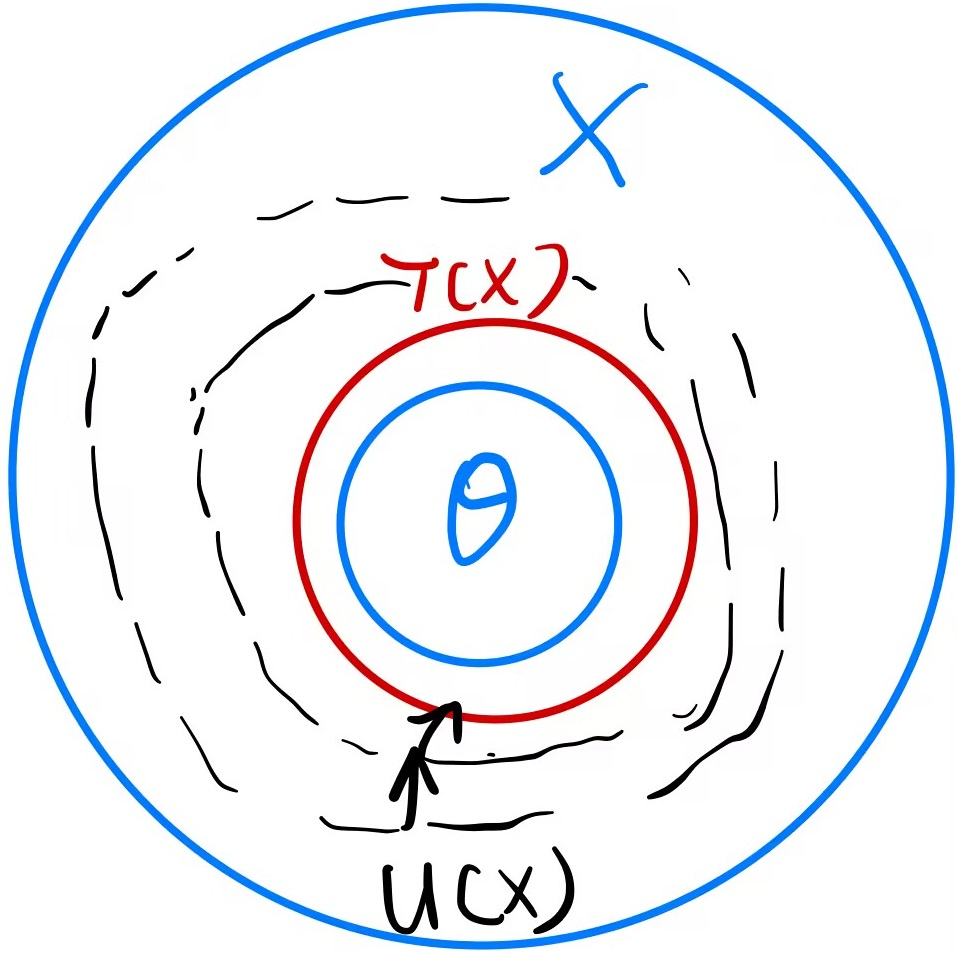
\includegraphics[width=0.41\textwidth]{./figures/chapter1/minimum_sufficient_statistic.png}
\end{figure}
\end{definition}

\begin{proposition}
$T(X),U(X)$ are the sufficient statistic, so
\begin{align*}
I(\theta;T(X)) &= I(\theta;X) \\
I(\theta;U(X)) &= I(\theta;X)
\end{align*}
$T(X)$ is the minimal sufficient statistic, so from data processing inequality:
$$I(X;T(X))\leq I(X;U(X))$$
understanding: 从上面的关系图来看, $T(X)$是对$U(X)$进行不断提纯,仅可能的去掉和$X$相关的信息, 只保留和$\theta$相关的信息.

e.g. 图像分类, 最理想的情况下, $(X,Y)$ 的最小充分统计量是$T(X)=Y$.
\end{proposition}